\chapter{Experiments with RTAB-Map} \label{experiments_rtab_map}

\section{Overview}

In this chapter we transition to using RTAB-Map for real-time mapping on the Turtlebot4, running ROS2. This involved extensive testing of the RTAB-Map with the OAK-D camera to assess its effectiveness and identify any limitations, particularly in terms of speed and orientation tracking.

Since the Turtlebot4 is running ROS2 I needed to find a tool that can do the mapping and runs on the said framework. In this semester we have tried RTAB-Map (Real-Time Appearance-Based Mapping)\cite{RTAB_Map_docs} for mapping.

\section{RTAB-Map using OAK-D}

First I tried out RTAB-Map with the OAK-D camera. It can be launched with the following command:
\FloatBarrier
\begin{lstlisting}[language=bash,frame=single,float=!ht]
$ ros2 launch depthai_ros_driver rtabmap.launch.py
\end{lstlisting}

The launched tool's UI can be seen on Figure \ref{fig:rtabmap_ros}. The top left panel shows the last keyframe captured by the camera, under it we can see the actual image recorded by it. On the right we can inspect the built map. This figure only serves to illustrate the UI of the tool, not the construction of the map, so the output is not spectacular.

\begin{figure}[htbp]
	\centering
	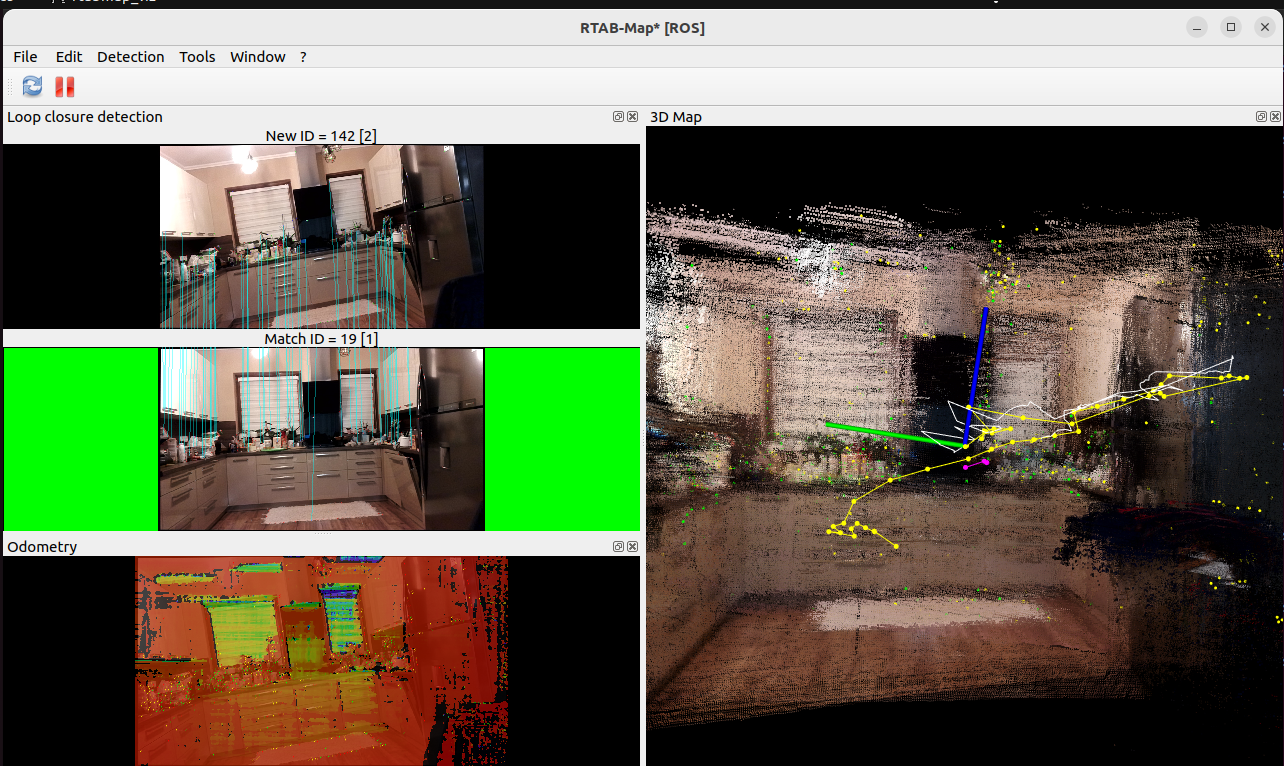
\includegraphics[width=150mm, keepaspectratio]{figures/rtabmap_ros.png}
	\caption{RTAB-Map ROS2}
	\label{fig:rtabmap_ros}
\end{figure}

When the device loses its orientation, it shows the last known position on the bottom left panel. When this happens the mapping stops and we have to navigate back to the exact same position where we lost track to get back on it and continue with the mapping. This is a huge downside of the application because this can happen quite a lot (especially in poor light). Furthermore, we sometimes had to restart the entire mapping process because, although we returned the camera to the last known position, RTAB-Map could not recognise it. Another disadvantage of the tool is its speed; the camera's image lags significantly.

To summarize our experiments, we only tried RTAB-Map while holding the camera by hand, moving and turning very slowly. However, due to the lag and loss of orientation, it was problematic to create a map even in a small room (seen on Figure~\ref{fig:rtabmap_nokia}, it can be seen that a lot of irrelevant points are added to the map making it unclear). We believe this issue may persist in the future if we use it on the actual robot, which can turn at high angular speeds. It will likely always lose track, and navigating back to the last known position will be time-consuming and only moderately successful.

\begin{figure}[H]
	\centering
	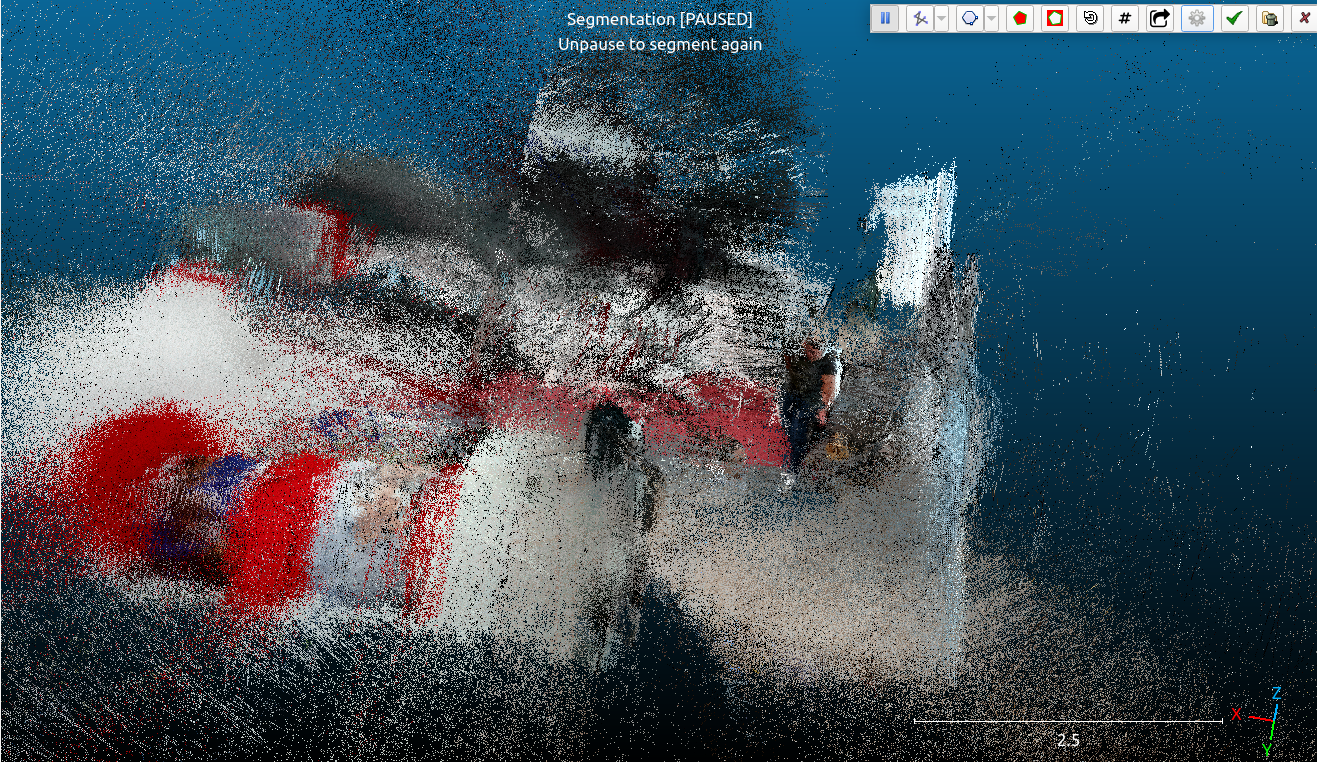
\includegraphics[width=150mm, keepaspectratio]{figures/rtabmap_nokia_office.png}
	\caption{RTAB-Map ROS generated map of the Nokia office, camera hold by hand}
	\label{fig:rtabmap_nokia}
\end{figure}

\FloatBarrier
\section{RTAB-Map iOS}

We tried the iOS version of RTAB-Map as a matter of interest and it worked more effectively than the ROS version with the OAK-D camera. I used the same iPhone 13 Pro as with the Luma AI (as seen on Figure~\ref{fig:luma_ai_szotyi_toy}). This app can create a mesh or a photorealistic map of our surrounding. When I generated a map it was running much smoother than the ROS version: it was not lagging at all and did not lost track even in rooms with poor light. A generated mesh map can be seen on Figure~\ref{fig:rtabmap_ios}.

\begin{figure}[htbp]
	\centering
	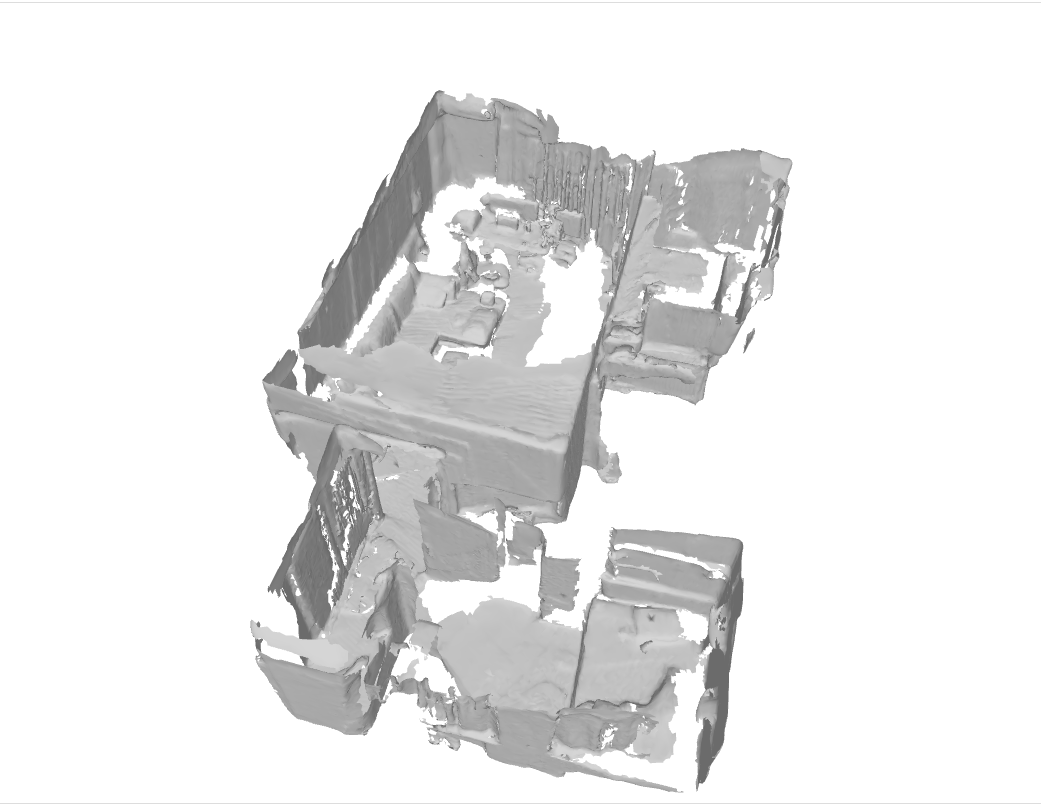
\includegraphics[width=150mm, keepaspectratio]{figures/rtabmap_ios.png}
	\caption{RTAB-Map iOS generated mesh map}
	\label{fig:rtabmap_ios}
\end{figure}

The holes in the floor are visible because the dark brown laminate reflected the light coming through the window. This made the area that RTAB-Map did not recognize light up due to the diversity of colors.
